\documentclass[conference]{IEEEtran}
\usepackage[utf8]{inputenc}
\usepackage[T1]{fontenc}
\usepackage{amsmath,amssymb}
\usepackage{graphicx}
\usepackage{booktabs}
\usepackage{microtype}
\usepackage{hyperref}
\usepackage{siunitx}
\sisetup{detect-all,group-digits=false}
\hypersetup{colorlinks=true,linkcolor=black,citecolor=black,urlcolor=blue}

\begin{document}

\title{Assignment 3: Thread Scaling in Shared-Memory Matrix Multiplication}
\author{\IEEEauthorblockN{Abel Castro Villar}
\IEEEauthorblockA{Data Science and Engineering\\Universidad de Las Palmas de Gran Canaria (ULPGC)\\Las Palmas de Gran Canaria, Spain\\\url{https://github.com/abelcasv/Assignment03_Abel}}}
\maketitle

\begin{abstract}
This study asks how OpenMP thread count affects the runtime and memory use of dense square matrix multiplication, and when parallel execution helps on one hybrid CPU. A C11 loop-interchanged kernel is compared with its sequential counterpart on identical binary64 inputs for six dimensions and eight requested team sizes. Each configuration has one warm-up and five measured repetitions; results are reported as medians and interquartile ranges. For $n=2000$, the median time falls from \SI{15.259}{\second} sequentially to \SI{1.377}{\second} with 12 OpenMP threads ($11.08\times$ speedup; $92.4\%$ efficiency). The OpenMP one-thread run is slower than the sequential baseline at this size. Scaling is not monotonic at every size, and a secondary blocked algorithm has a different thread-count profile. The evidence supports parallel execution for the larger tested matrices on this host, but does not identify individual core placement or establish a universal optimum.
\end{abstract}

\begin{IEEEkeywords}
OpenMP, matrix multiplication, thread scaling, speedup, efficiency, reproducible benchmarking.
\end{IEEEkeywords}

\section{Introduction}
Dense matrix multiplication is a useful workload for studying shared-memory parallelism because its arithmetic work grows as $O(n^3)$ while three dense $n\times n$ binary64 arrays require $24n^2$ bytes. This report follows Assignment 3's requirement to compare equivalent sequential and parallel implementations, vary thread count, validate correctness, and report time and memory with enough detail to reproduce the measurements~\cite{courseproposal}.

\subsection{Question and hypotheses}
The research question is: \emph{How does OpenMP team size affect runtime and memory use for dense matrix multiplication, and at which tested matrix sizes does the parallel version outperform its sequential counterpart on this host?} The primary comparison uses the same loop-interchanged algorithm in both implementations. Before measurement, we expected small workloads to be sensitive to parallel-region overhead, larger workloads to benefit from multiple threads, and performance to stop improving once thread count exceeded the available execution contexts. These are predictions; the results below test them and do not assume them to be true.

\section{Methods}
\subsection{Implementations and inputs}
The primary sequential kernel and its OpenMP counterpart use row-major \texttt{double} arrays and the same $i$-$k$-$j$ loop order. The OpenMP version statically distributes the outer $i$ loop; each iteration writes a separate row of $C$, avoiding shared writes to the same output elements. A second, blocked implementation uses $32\times32$ tiles, a common locality technique for matrix multiplication~\cite{goto}, and is compared only with its own sequential version. It is a secondary algorithm comparison, not a substitute baseline. Matrix input is shared by every method at a given size.

The generator uses Python's \texttt{random.Random(42)} stream, draws each element using \texttt{random()} in $[0,1)$, and writes six decimal places to CSV. Rounding can produce stored values of \texttt{1.000000}; the observed CSV range is $[0,1]$. Values are read as IEEE 754 binary64. The six dimensions are $n\in\{250,500,750,1000,1500,2000\}$. The generator, fixtures and matrix files can be recreated by the commands in the README. The script writes \texttt{data/SHA256SUMS.txt}, a checksum manifest for the 12 dense inputs and five correctness fixtures; dense matrices are excluded from version control. Python documents this generator as using Mersenne Twister; reproducibility here is tied to the included generator and saved stream, not to matching random sequences in other languages~\cite{pythonrandom}.

\subsection{Host and execution configuration}
The recorded host has an Intel Core i5-1335U, 10 physical cores (2 Performance-cores and 8 Efficient-cores), 12 logical processors, and \SI{15.63}{\gibi\byte} total physical memory. The core and thread counts are from the processor specification~\cite{intelspec}; no memory-module type or speed was measured. The operating system is Windows build 26300. The code was compiled with MSYS2 UCRT64 GCC 16.1.0 using \texttt{-Wall -Wextra -O3 -std=c11 -fopenmp -march=native}. The compiler reports OpenMP 5.2 compatibility (\texttt{\_OPENMP=202111})~\cite{openmp52}.

Requested OpenMP team sizes were $p\in\{1,2,4,8,10,12,16,24\}$. The measured team size matched the requested size in all OpenMP records. The program disabled dynamic adjustment; the run set \texttt{OMP\_PROC\_BIND=false} and left \texttt{OMP\_PLACES} unset. No explicit affinity was used, so counts of 10 or 12 do not establish which P- or E-cores ran the workers. Requests above 12 are labelled oversubscribed relative to the host's logical processor count.

\subsection{Timing, memory and correctness}
Inputs are loaded and arrays allocated outside timing. A monotonic timer (Windows \texttt{QueryPerformanceCounter}) surrounds one kernel call. It therefore includes zero-initialisation of $C$ and, for OpenMP, parallel-team and loop overhead; it excludes file input, allocation, and a subsequent checksum over every output element. The checksum is consumed through a volatile sink. The same boundary is used for each sequential/OpenMP pair. One warm-up is excluded, followed by five measured repetitions per configuration. Raw samples are retained. The reported statistic is the median; quartiles are NumPy's 25th and 75th percentiles, and IQR is $Q_3-Q_1$.

The program checks known-answer, identity and zero $4\times4$ fixtures, then checks all kernels and tested OpenMP sizes against a trusted $n=250$ reference. A result passes when $|x-y|\le10^{-4}+10^{-4}|y|$. The complete benchmark repeated these checks successfully. A per-repetition 120-second stop threshold and a three-array structural-storage budget of 2048 MiB were set before the full run. The stop threshold is checked after a call returns: an over-budget sample would be retained and the remaining repetitions for that configuration skipped. The largest size tested was $n=2000$; larger sizes were not attempted. No call exceeded the time threshold, and no size exceeded the storage budget. The budget is an estimate of matrix-array storage, not a measured cap on total process memory.

The program records Windows process peak working set using \texttt{GetProcessMemoryInfo}. This API reports current or peak process working-set values~\cite{msmemory}. Since all configurations run in one process and this metric is a high-water mark, the CSV values cannot be interpreted as independent per-configuration memory peaks. I report the observed overall peak and the per-size structural estimate separately.

\section{Results}
The validated dataset contains 540 observations: 108 configurations, each with five repetitions. It covers six sizes, two algorithms (loop-interchanged and blocked), and eight OpenMP team sizes, with one matched sequential configuration per algorithm and size. All 12-thread and oversubscribed requests created the recorded team size; no sample was excluded. The analysis script checks the raw schema, full configuration grid, repetition counts, duplicates, finite positive times, actual team sizes and oversubscription flags before producing the summary.

\subsection{Primary thread-scaling comparison}
Table~\ref{tab:size_scaling} shows the sequential baseline and the 12-thread primary kernel at representative sizes. For $n=2000$, the median falls from \SI{15.259}{\second} to \SI{1.377}{\second}, a matched speedup of $11.08\times$. At $n=500$, the speedup is $3.77\times$; at $n=1500$, it is $3.89\times$. Results do not increase smoothly with size: variability in the sequential $n=1000$ sample is large, and the 12-thread speedup at $n=1500$ is lower than at $n=1000$ or $n=2000$. Accordingly, the comparison is reported per size rather than described by a single scaling trend.

\begin{table*}[t]
\caption{Sequential baseline and matched 12-thread OpenMP \texttt{ikj} results. Times are median [Q1, Q3] in seconds.}
\label{tab:size_scaling}
\centering
\small
\begin{tabular}{rrrrr}
\toprule
$n$ & $T_{seq}$ & $T_{12}$ & $S(12)$ & $E(12)$ \\
\midrule
500  & 0.0595 [0.0590, 0.0641] & 0.0158 [0.0157, 0.0182] & 3.77 & 31.5\% \\
1000 & 1.2341 [1.0738, 1.6746] & 0.2079 [0.2069, 0.2115] & 5.93 & 49.5\% \\
1500 & 3.2699 [3.1973, 3.2991] & 0.8397 [0.8164, 0.9137] & 3.89 & 32.5\% \\
2000 & 15.2589 [14.2205, 15.9683] & 1.3768 [1.3105, 1.3896] & 11.08 & 92.4\% \\
\bottomrule
\end{tabular}
\end{table*}

The OpenMP one-thread configuration exposes implementation overhead. Relative to sequential \texttt{ikj}, its median is about 0.9\% slower at $n=250$, 7.5\% slower at $n=500$, 12.8\% slower at $n=750$, and 100.5\% slower at $n=1500$. At $n=1000$ and $n=2000$ it is respectively 19.8\% and 7.3\% faster in these samples. The mixed direction and the high IQR at $n=1000$ mean that one-thread overhead is not a fixed penalty; runtime and system-state variation affect the observed comparison.

\begin{figure*}[t]
\centering
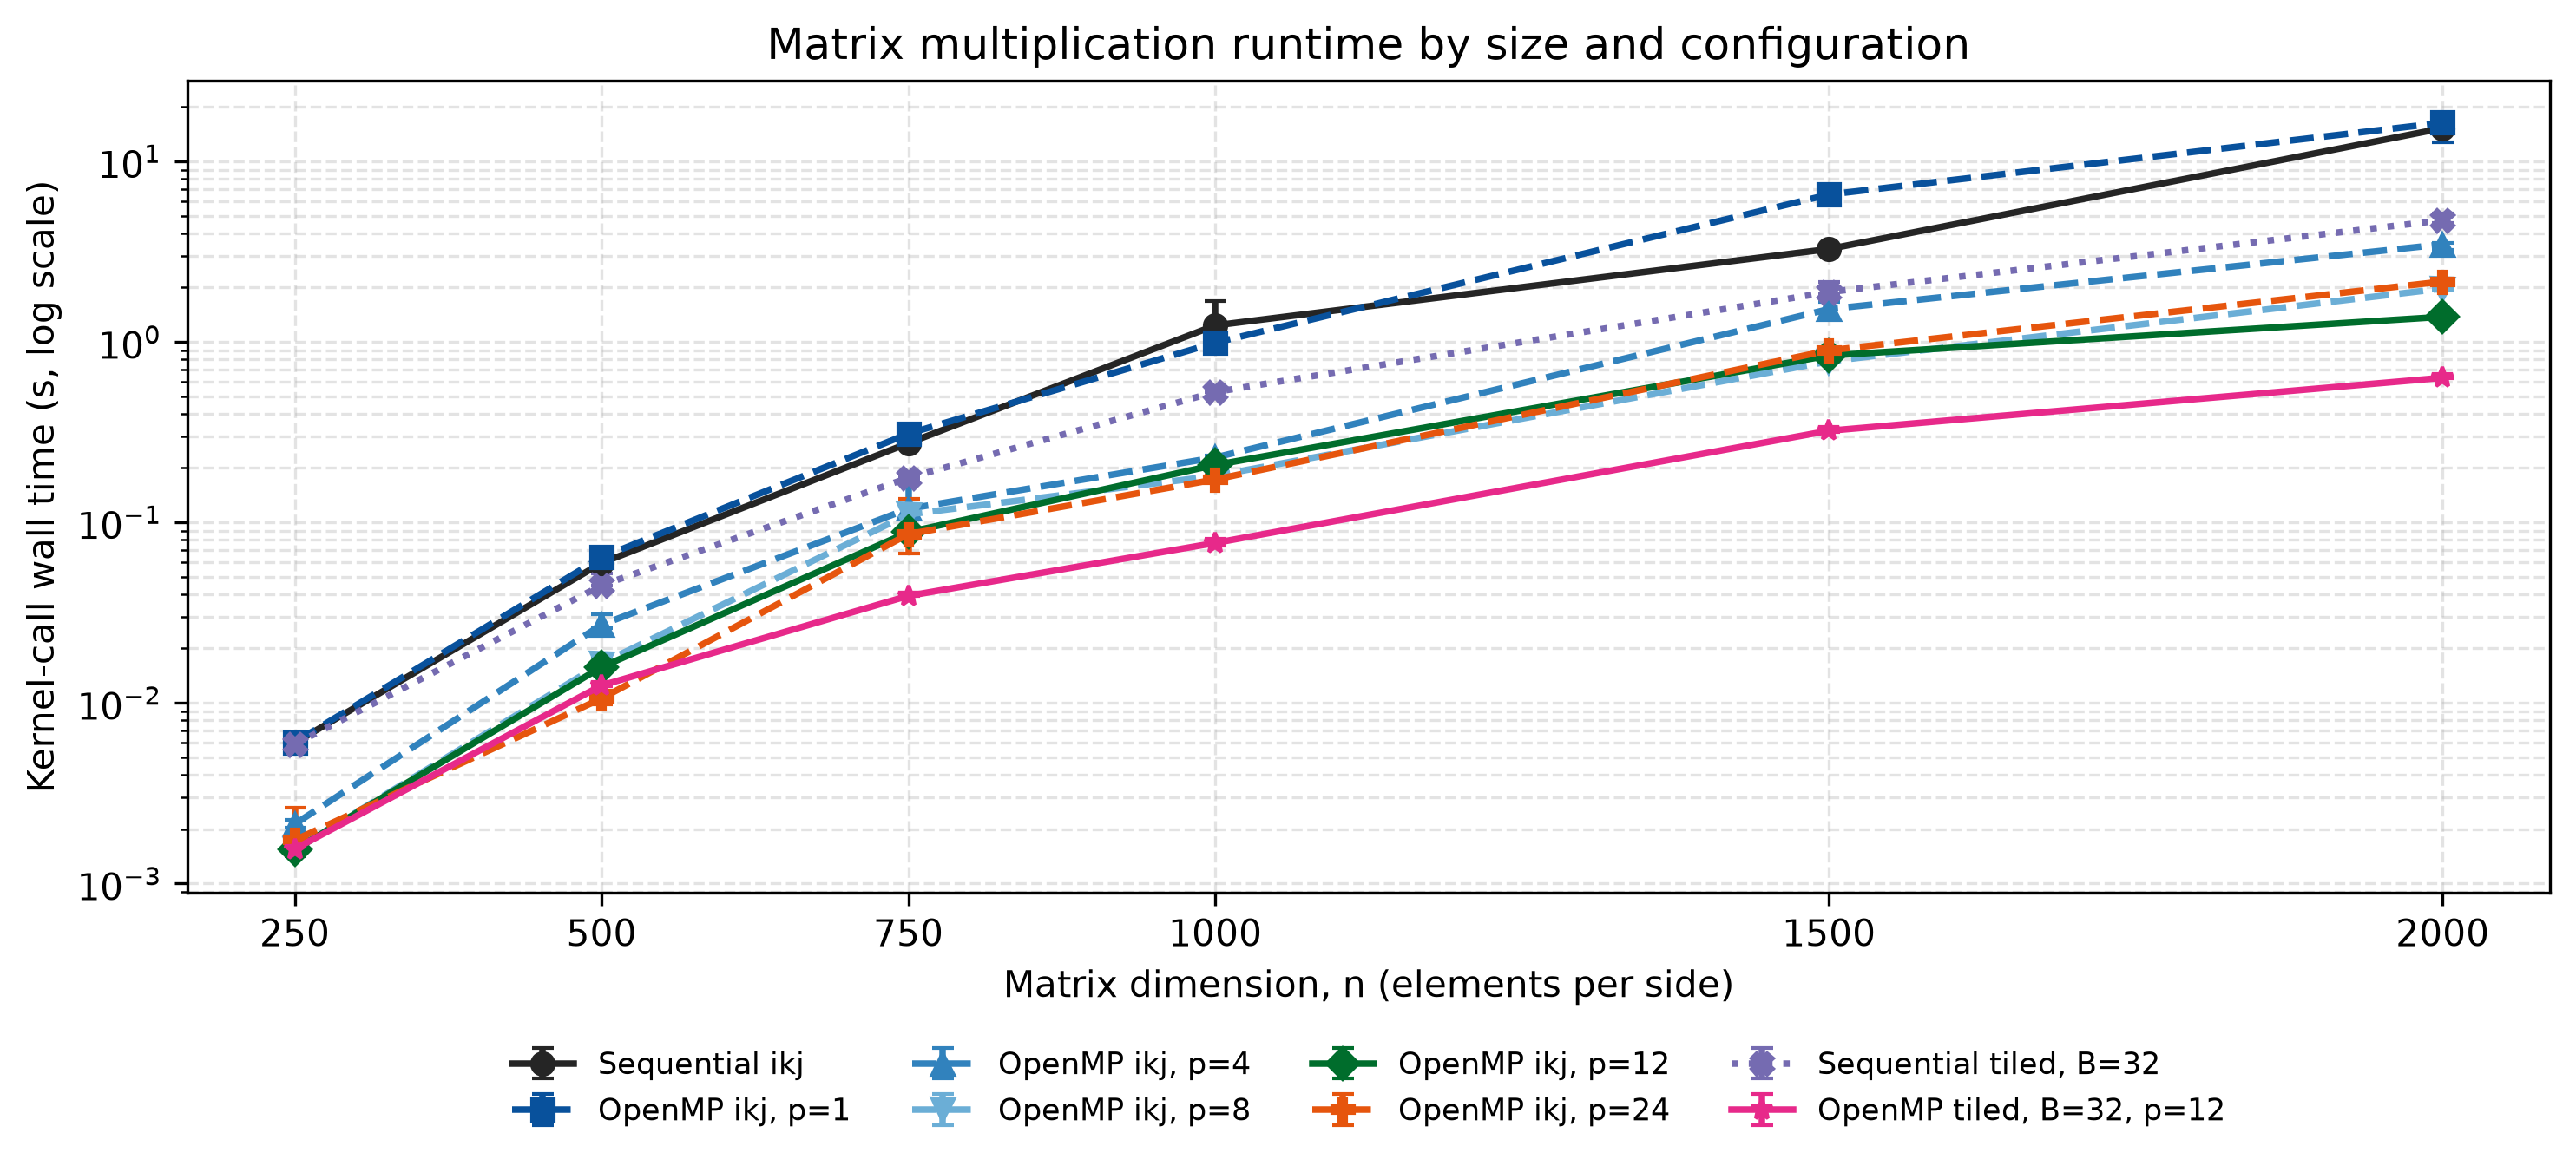
\includegraphics[width=0.92\textwidth]{plots/parallel_runtime_scaling.png}
\caption{Runtime medians and interquartile ranges by matrix size for selected sequential and OpenMP configurations. The vertical axis is logarithmic.}
\label{fig:runtime}
\end{figure*}

At $n=2000$, primary-kernel speedup increases from $0.93\times$ with one OpenMP thread to $11.08\times$ with 12 threads, then falls to $6.62\times$ at 16 and $7.07\times$ at 24. The 12-thread configuration is the best observed primary-kernel median in this size. The 16- and 24-thread results are slower than the 12-thread result, but the 24-thread median is slightly faster than the 16-thread median; oversubscription therefore does not produce a strictly monotonic penalty in these measurements.

\begin{table*}[t]
\caption{Primary \texttt{ikj} scaling at $n=2000$. Times are median [Q1, Q3] in seconds.}
\label{tab:thread_scaling}
\centering
\small
\begin{tabular}{rrrr}
\toprule
$p$ & $T_p$ & $S(p)$ & $E(p)$ \\
\midrule
1  & 16.3745 [12.8002, 17.4957] & 0.93 & 93.2\% \\
2  & 5.8807 [3.8517, 7.6126] & 2.59 & 129.7\% \\
4  & 3.4712 [3.2525, 3.5302] & 4.40 & 109.9\% \\
8  & 1.9744 [1.9540, 1.9768] & 7.73 & 96.6\% \\
10 & 1.5443 [1.4599, 1.5939] & 9.88 & 98.8\% \\
12 & 1.3768 [1.3105, 1.3896] & 11.08 & 92.4\% \\
16 & 2.3040 [1.6423, 2.5708] & 6.62 & 41.4\% \\
24 & 2.1583 [2.0985, 2.2466] & 7.07 & 29.5\% \\
\bottomrule
\end{tabular}
\end{table*}

The $p=2$ and $p=4$ medians exceed ideal linear efficiency (100\%). The team sizes were verified, inputs and timing boundary were matched, all five samples were retained, and correctness passed. However, the $p=2$ IQR is wide, and no hardware counters, frequency logs, or core affinity were collected. A cache, frequency, or scheduler explanation is plausible but not demonstrated by these data; the superlinear values should be treated as an observation requiring further controlled investigation, not as evidence of a specific mechanism.

\begin{figure*}[t]
\centering
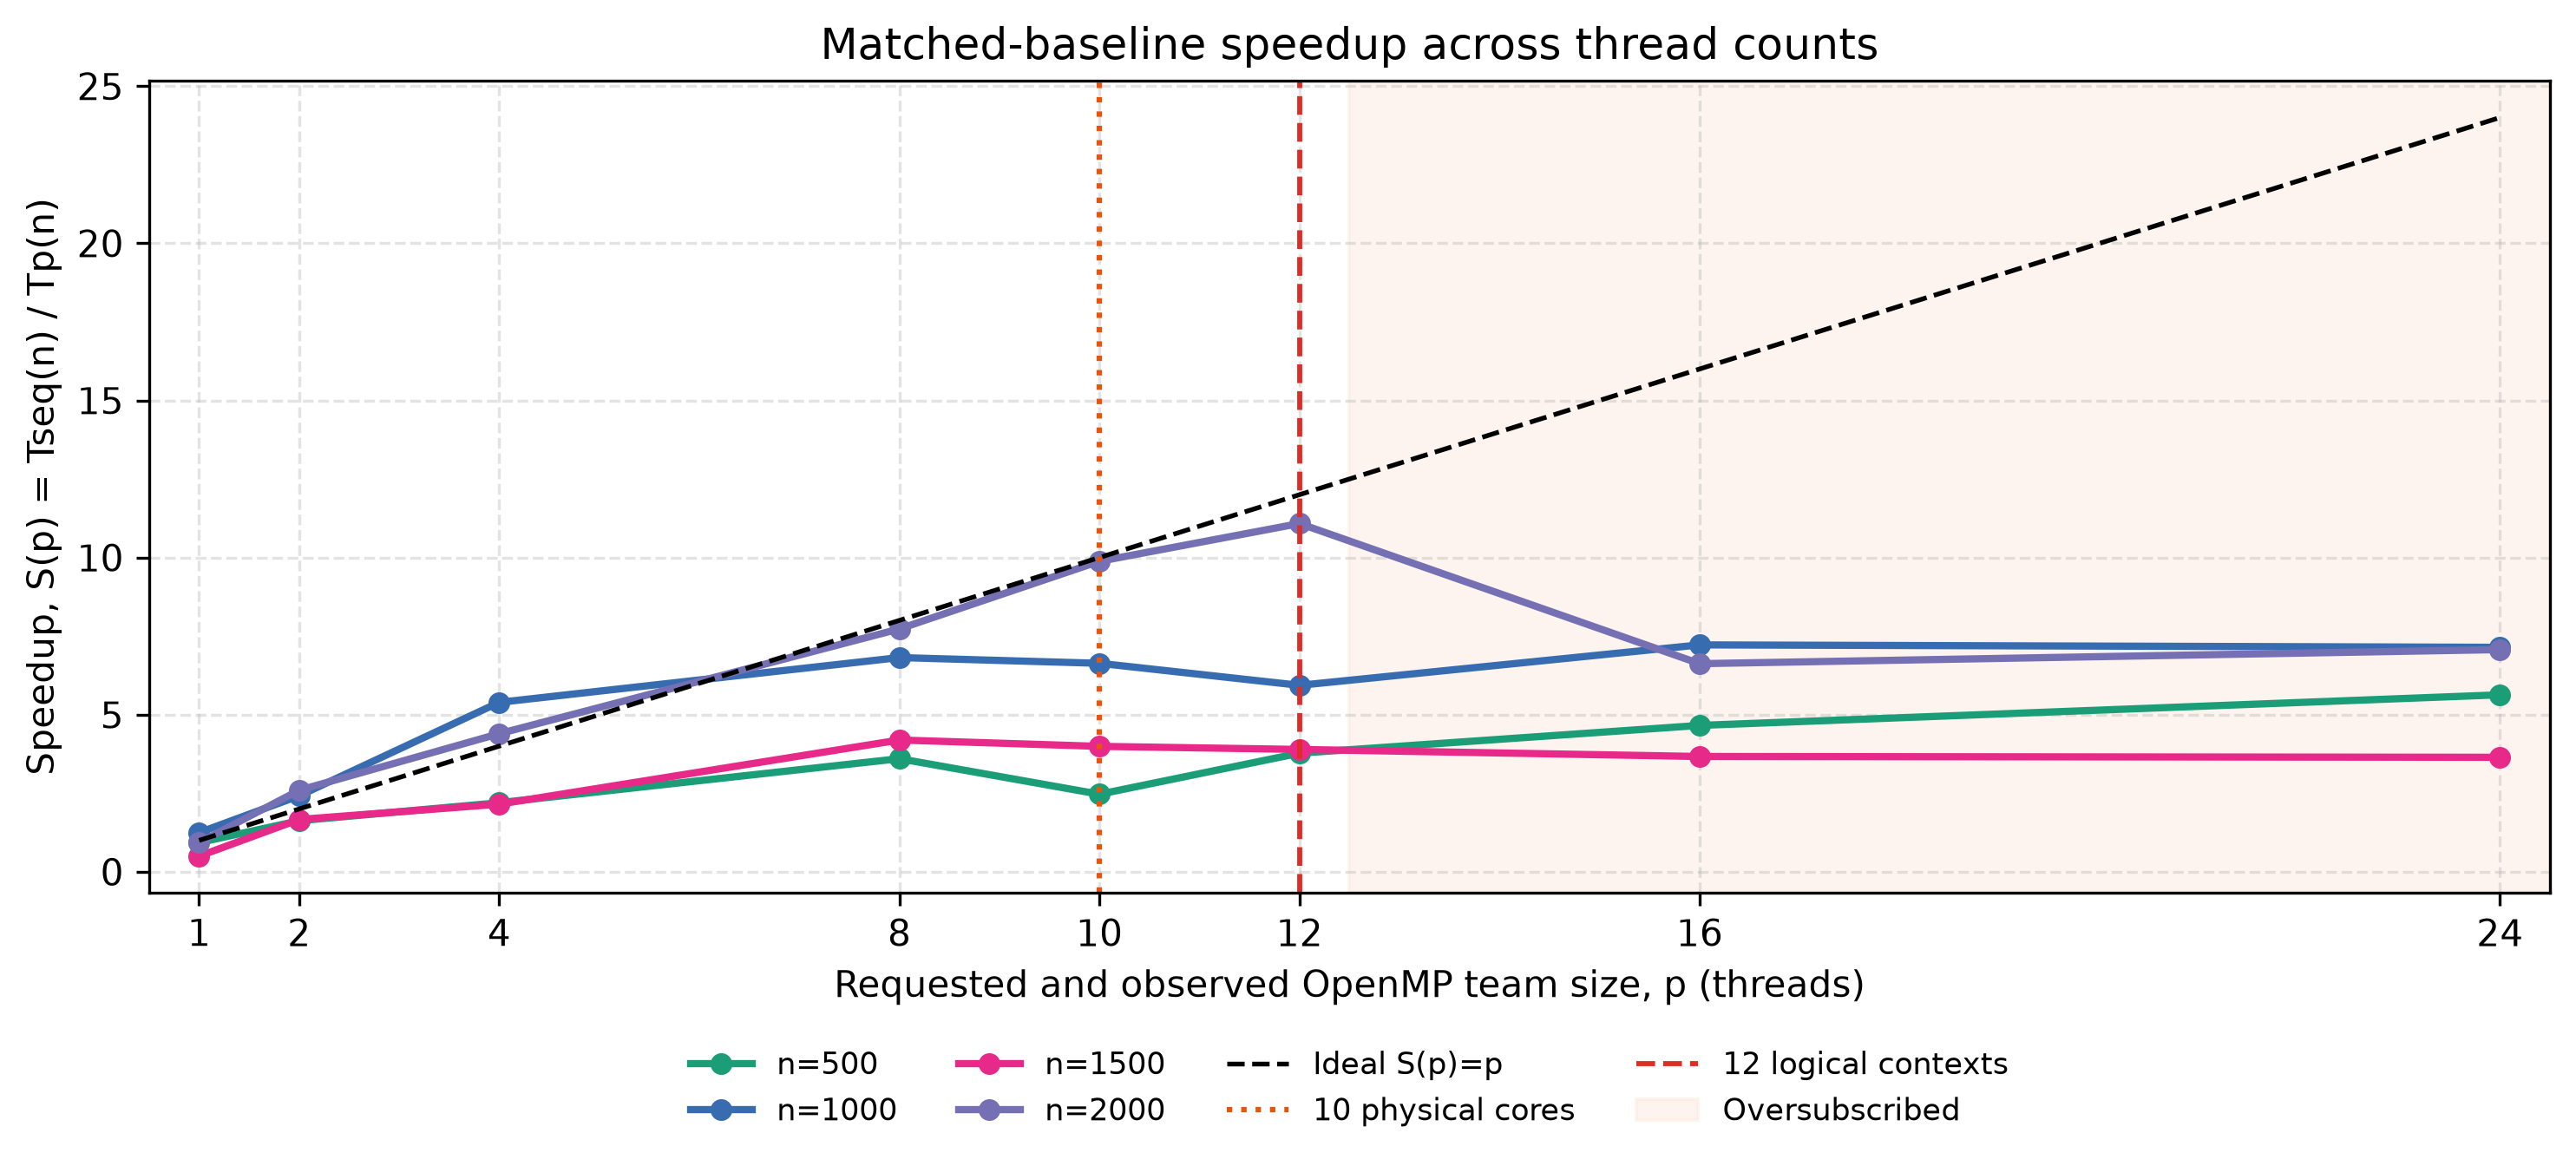
\includegraphics[width=0.92\textwidth]{plots/parallel_speedup_curves.png}
\caption{Matched-baseline speedup for the primary kernel. The dashed line is ideal linear speedup; vertical markers denote physical-core and logical-processor counts, not observed worker placement.}
\label{fig:speedup}
\end{figure*}

\begin{figure*}[t]
\centering
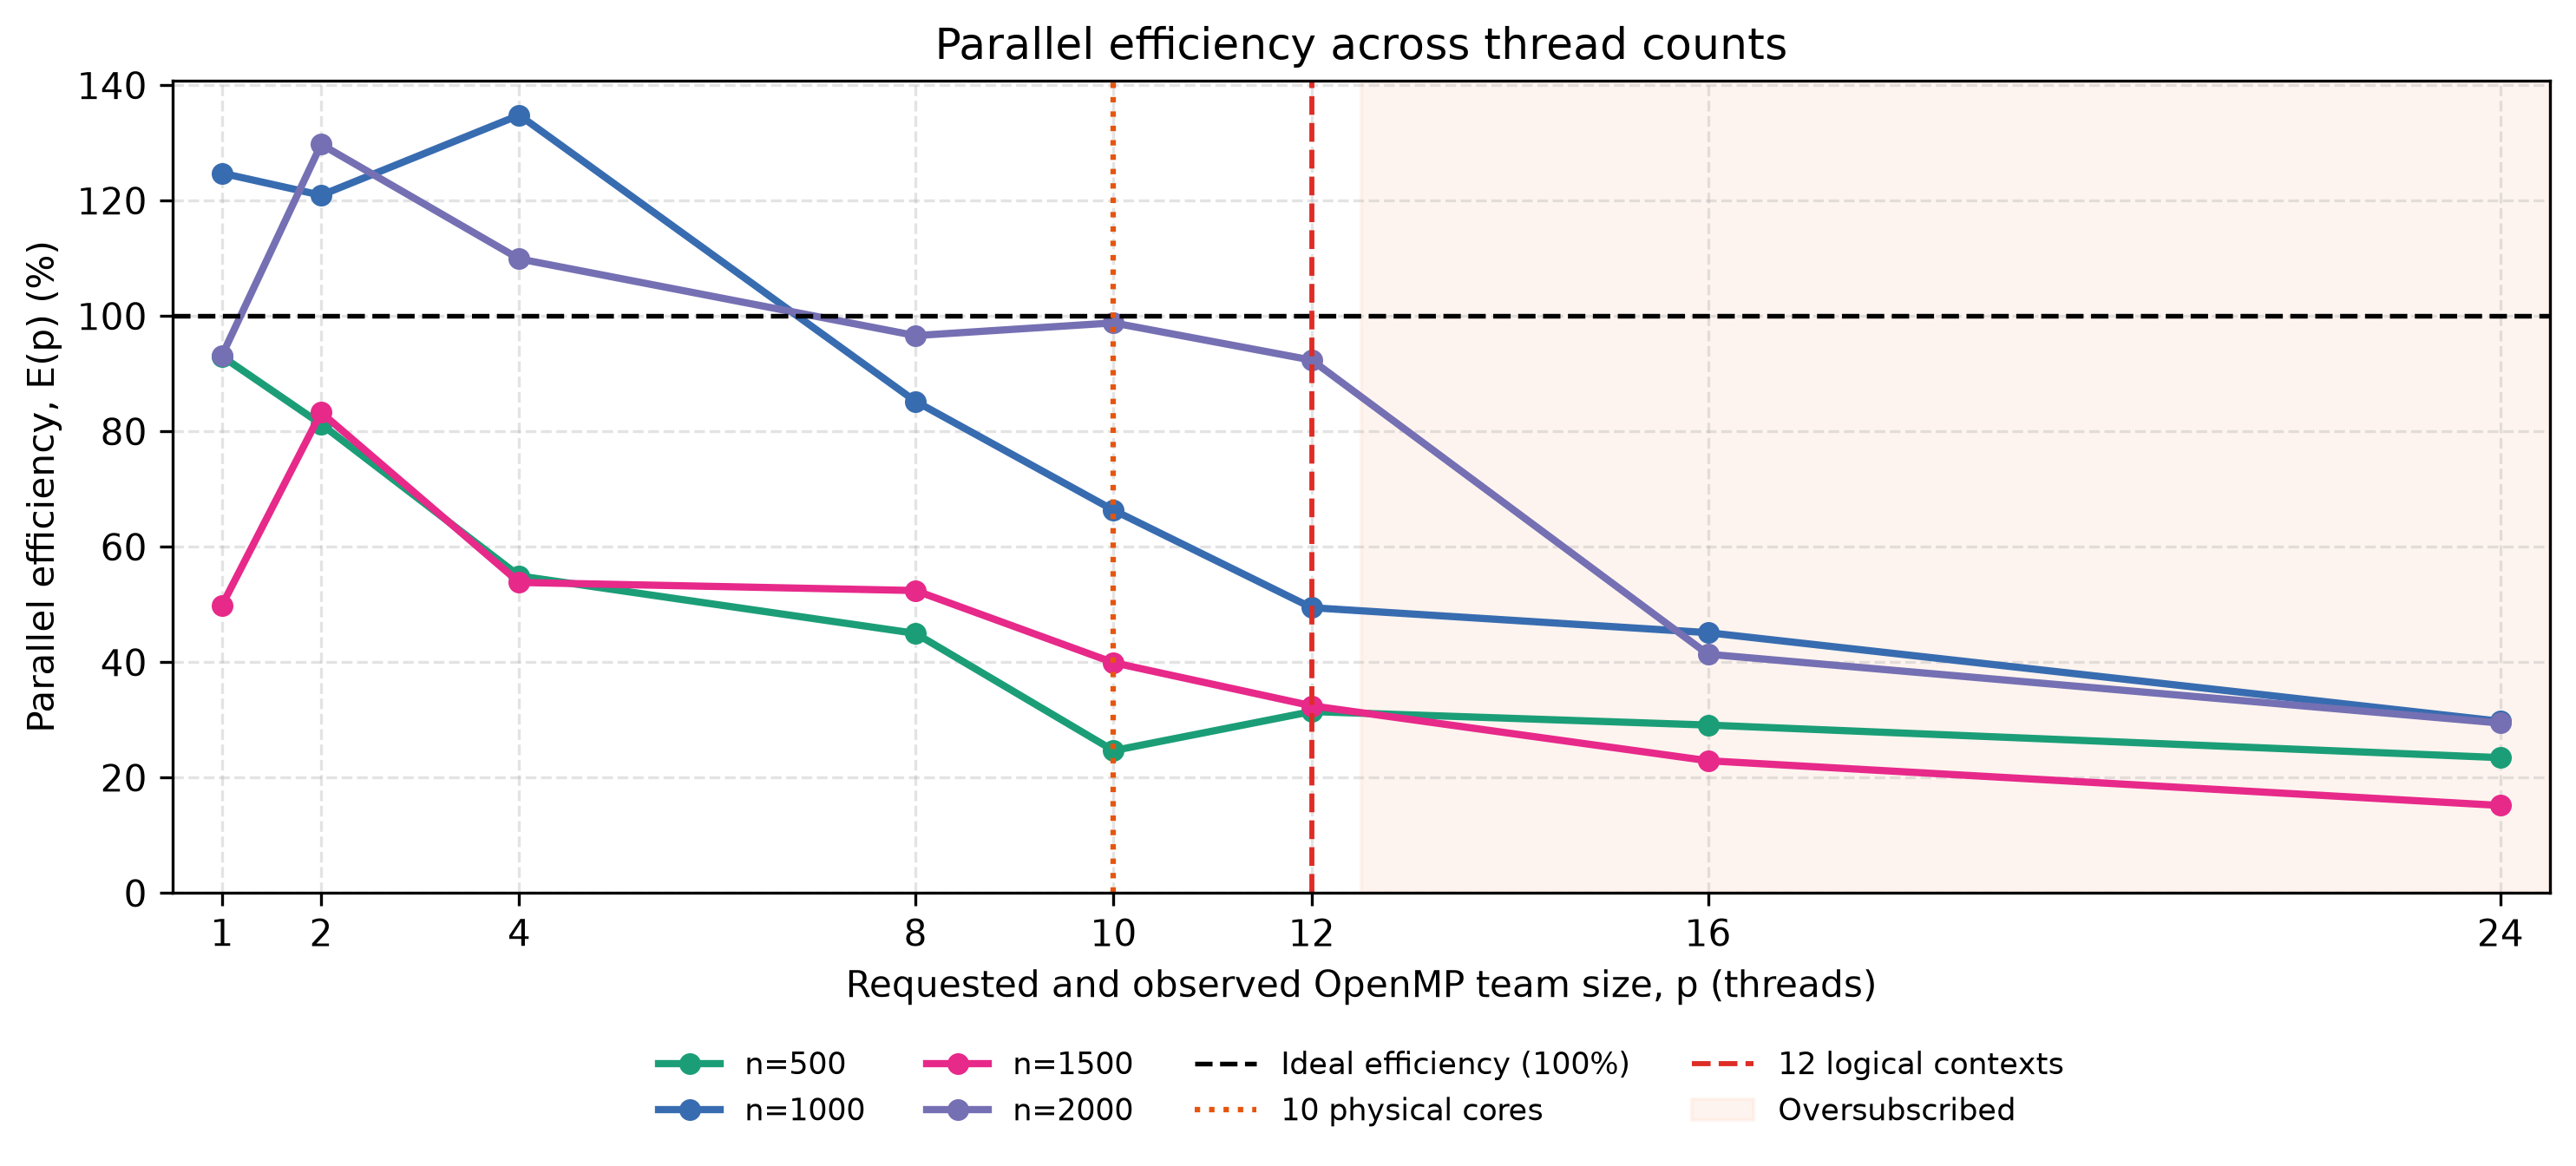
\includegraphics[width=0.92\textwidth]{plots/parallel_efficiency_curves.png}
\caption{Efficiency $E(p)=S(p)/p$ for the primary kernel. Values above 100\% are visible and discussed rather than clipped. Shading marks requests above 12 logical processors.}
\label{fig:efficiency}
\end{figure*}

\subsection{Secondary blocked-kernel comparison and memory}
At $n=2000$, the sequential blocked kernel has a median of \SI{4.7202}{\second}, compared with \SI{15.2589}{\second} for the sequential loop-interchanged kernel. This is evidence that the two algorithms have different performance on this host; it is not a pure thread-count effect. The blocked OpenMP kernel reaches \SI{0.6026}{\second} at $p=8$ and \SI{0.5826}{\second} at $p=24$. The latter is the fastest observed blocked configuration despite being oversubscribed, while $p=16$ is slower. The small difference between $p=8$ and $p=24$ should be interpreted cautiously and does not support a general claim that oversubscription helps.

Three matrices at $n=2000$ occupy an estimated \SI{91.55}{\mebi\byte}; the observed process high-water working set across the complete run is \SI{97.36}{\mebi\byte}. Structural estimates for $n=500$, 1000, 1500 and 2000 are respectively 5.72, 22.89, 51.50 and \SI{91.55}{\mebi\byte}. The process-level working-set value includes runtime and other resident pages and is cumulative across the process; it cannot be compared row-by-row as if it were a fresh per-configuration measurement. No configuration exceeded the stated structural memory budget.

\section{Discussion and limitations}
The required equivalent comparison answers the research question within the tested scope: for $n=2000$, the 12-thread OpenMP implementation is substantially faster than its sequential counterpart, while the OpenMP one-thread case is not faster. For smaller sizes, results vary: the smallest cases include short measured calls, and the $n=1000$ sequential baseline has a broad IQR. These observations caution against generalising from one size or selecting a thread count using runtime alone without considering variability.

Efficiency and time do not decline monotonically as thread count rises. At $n=2000$, performance is best at 12 threads for the primary kernel, with slower medians at 16 and 24; in the blocked extension, the fastest observed median is at 24. The data establish those observations but cannot isolate thread scheduling, thermal state, processor frequency, or P/E-core placement as causes. Repeated runs on a controlled system with recorded affinity and performance counters would be needed to make those causal claims.

The study has five repetitions per configuration and one full run on a single Windows host. The process-wide peak-working-set metric is not a per-configuration peak. Inputs are rounded to six decimal places by the generator; output is checked with explicit absolute and relative tolerances. The tested range ends at $n=2000$, and no conclusion is made for larger matrices or other processors. The blocked kernel is secondary. SIMD vectorisation is optional under the assignment and is deliberately excluded from the final core results; no SIMD performance conclusion is drawn.

\section{Conclusion}
The main comparison uses identical input matrices, data representation and loop order for sequential and OpenMP kernels, validates correctness, and records five repetitions for each of 108 configurations. At the largest tested dimension, $n=2000$, 12 OpenMP threads reduce the median primary-kernel time from \SI{15.259}{\second} to \SI{1.377}{\second} ($11.08\times$ speedup and $92.4\%$ efficiency). The OpenMP one-thread result reveals non-constant framework/runtime effects; oversubscribed configurations are slower than the 12-thread primary result but do not form a monotonic trend. These conclusions apply to the measured implementation and host only. The raw CSV, deterministic input generator, analysis script, environment records, exact commands and report source are included in the repository.

\section*{AI assistance declaration}
Gemini was used to draft the initial \texttt{CLAUDE.md} project guidance and prompt plan. Claude was used to carry out implementation and documentation work through those prompts. OpenAI Codex was used for an independent audit and subsequent corrections to the benchmark, analysis, reproducibility materials and this report. AI-generated material is not evidence; the student remains responsible for understanding and defending the code, measurements, interpretation and references.

\begin{thebibliography}{6}
\bibitem{courseproposal} Big Data Course Team, ``BIG DATA | Individual Assignments | Revised proposal 2026--2027,'' Assignment 3 and common experimental protocol, course document supplied for the assignment, 2026.
\bibitem{openmp52} OpenMP Architecture Review Board, \emph{OpenMP Application Programming Interface Version 5.2}, Nov. 2021. [Online]. Available: \url{https://www.openmp.org/spec-html/5.2/openmp.html}.
\bibitem{intelspec} Intel Corporation, ``Intel Core i5-1335U Processor Specifications.'' [Online]. Available: \url{https://www.intel.com/content/www/us/en/products/sku/232153/intel-core-i51335u-processor-12m-cache-up-to-4-60-ghz/specifications.html}. Accessed: Nov. 1, 2026.
\bibitem{pythonrandom} Python Software Foundation, ``random --- Generate pseudo-random numbers,'' Python 3 documentation. [Online]. Available: \url{https://docs.python.org/3/library/random.html}. Accessed: Nov. 1, 2026.
\bibitem{msmemory} Microsoft, ``Process Memory Usage Information,'' Windows API documentation. [Online]. Available: \url{https://learn.microsoft.com/en-us/windows/win32/psapi/process-memory-usage-information}. Accessed: Nov. 1, 2026.
\bibitem{goto} K. Goto and R. A. van de Geijn, ``Anatomy of high-performance matrix multiplication,'' \emph{ACM Transactions on Mathematical Software}, vol. 34, no. 3, Article 12, 2008, doi: 10.1145/1356052.1356053.
\end{thebibliography}

\end{document}
